% !TeX program = xelatex
% project_id: guardsynth-coc
% Updated 2026-10-20: current NCA Introduction, terminology, and document-grounded SMT results.
% Inputs: NCA 01-introduction-v03-en.tex; 03-method.tex; 05-results.tex.
% Composition: paper1-constraint-composition-001/document-grounded-composition-2026-10-17-002/RESULT.json.
% No new experiments or model predictions; source evidence reviewed in that frozen run.
% White slides with dark text, accent labels, and lightly outlined boxes.
% Compile beside this source; see README.md for the local TeX dependency path.
\documentclass[aspectratio=169,11pt]{beamer}
\usepackage{lmodern,fontspec}
\setsansfont{TeX Gyre Heros}
\setmainfont{TeX Gyre Heros}
\usefonttheme{professionalfonts}
\usepackage{amsmath,amssymb,tikz}
\usepackage{pgfplots}
\usetikzlibrary{arrows.meta}
\definecolor{navy}{HTML}{142D4E}
\definecolor{teal}{HTML}{087E8B}
\definecolor{muted}{HTML}{586776}
\definecolor{line}{HTML}{DCE5EA}
\setbeamercolor{normal text}{fg=navy,bg=white}
\setbeamertemplate{navigation symbols}{}
\setbeamertemplate{footline}{}
\hypersetup{
  pdftitle={Problem Definition for Language-Reasoning Driving Models},
  pdfsubject={Rule-conditioned learning, evidence-bound constraints, and bounded SMT composition checks},
  pdfauthor={GuardSynth research project},
  colorlinks=true,urlcolor=muted
}
\tikzset{
  textnode/.style={anchor=north west,inner sep=0pt,align=left,text=navy},
  panel/.style={draw=line,line width=0.55pt,fill=muted!3,rounded corners=1.5pt},
  focuspanel/.style={draw=teal!30,line width=0.65pt,fill=teal!4,rounded corners=1.5pt},
  arrow/.style={-{Stealth[length=2mm]},line width=0.8pt,draw=teal!60}
}
\pgfplotsset{
  compat=1.17,
  corebars/.style={
    ybar=3pt,bar width=8pt,scale only axis,
    width=5.35cm,height=2.65cm,
    xmin=0.5,xmax=3.5,ymin=0,
    xtick={1,2,3},xticklabels={Entry,Hold: max,Hold: XY},
    tick label style={font=\fontsize{7}{9}\selectfont,text=muted},
    axis lines=left,axis line style={draw=muted!50},
    ymajorgrids,grid style={draw=line,line width=0.3pt},
    tick style={draw=muted!50},clip=false,
    nodes near coords,
    every node near coord/.append style={
      font=\fontsize{7}{9}\selectfont,text=navy,
      /pgf/number format/fixed,/pgf/number format/precision=2,
      /pgf/number format/fixed zerofill
    }
  }
}
\begin{document}

\begin{frame}[plain]

\begin{tikzpicture}[remember picture,overlay,x=1cm,y=1cm]
\begin{scope}[shift={(current page.south west)}]
  \node[textnode,text=teal,font=\fontsize{8}{10}\selectfont]
    at (0.75,8.45) {TECHNOLOGY GAPS};
  \node[textnode,text width=14.5cm,font=\fontsize{20}{25}\selectfont\bfseries]
    at (0.75,7.86) {External Rules and Driving Behavior};
  \node[textnode,text width=14.5cm,text=muted,font=\fontsize{10.5}{14}\selectfont]
    at (0.75,7.02)
    {Changing the rule can change admissible actions in the same scene.};

  \node[textnode,text width=4.1cm,font=\fontsize{11}{14}\selectfont\bfseries]
    at (1.00,6.28) {01 | Reasoning and\\rule compliance};
  \node[textnode,text width=4.1cm,font=\fontsize{11}{14}\selectfont\bfseries]
    at (5.95,6.28) {02 | Interacting\\behavioral conditions};
  \node[textnode,text width=4.1cm,font=\fontsize{11}{14}\selectfont\bfseries]
    at (10.90,6.28) {03 | Formal meaning\\and model use};

  \foreach \left in {0.75,5.70,10.65} {
    \path[panel] (\left,3.20) rectangle ++(4.60,1.93);
    \path[focuspanel] (\left,0.92) rectangle ++(4.60,1.93);
  }
  \foreach \mid in {3.05,8.00,12.95} {
    \draw[arrow,line width=1pt] (\mid,3.10) -- (\mid,2.92);
  }
  \foreach \x in {1.00,5.95,10.90} {
    \node[textnode,text=teal,font=\fontsize{7.5}{10}\selectfont\bfseries]
      at (\x,4.88) {CURRENT PRACTICE};
    \node[textnode,text=navy,font=\fontsize{7.5}{10}\selectfont\bfseries]
      at (\x,2.63) {REMAINING GAP};
  }
  \node[textnode,text width=4.1cm,font=\fontsize{10}{13}\selectfont]
    at (1.00,4.48)
    {Models link scenes to\\language reasoning and\\predicted motion.};
  \node[textnode,text width=4.1cm,font=\fontsize{10}{13}\selectfont]
    at (5.95,4.48)
    {Policies combine facts,\\rule values, and\\model assumptions.};
  \node[textnode,text width=4.1cm,font=\fontsize{10}{13}\selectfont]
    at (10.90,4.48)
    {Language expresses\\timing, units, negation,\\and boundary conditions.};

  \node[textnode,text=navy,text width=4.1cm,font=\fontsize{10}{13}\selectfont]
    at (1.00,2.23)
    {An explained action\\may still violate a rule\\supplied at inference.};
  \node[textnode,text=navy,text width=4.1cm,font=\fontsize{10}{13}\selectfont]
    at (5.95,2.23)
    {Individually satisfiable\\conditions can become\\incompatible together.};
  \node[textnode,text=navy,text width=4.1cm,font=\fontsize{10}{13}\selectfont]
    at (10.90,2.23)
    {A sentence may alter\\checked meaning; model\\compliance is separate.};

  \draw[line,line width=0.4pt] (0.75,0.74) -- (15.25,0.74);
  \node[textnode,text=muted,font=\fontsize{7}{10}\selectfont]
    at (0.75,0.56) {Source: current NCA Introduction; technology context and three construction challenges.};
  \node[anchor=north east,inner sep=0pt,text=muted,font=\fontsize{7.5}{10}\selectfont]
    at (15.25,0.56) {\insertframenumber{} / \inserttotalframenumber};
\end{scope}
\end{tikzpicture}
\end{frame}

\begin{frame}[plain]
\begin{tikzpicture}[remember picture,overlay,x=1cm,y=1cm]
\begin{scope}[shift={(current page.south west)}]
  \node[textnode,text=teal,font=\fontsize{8}{10}\selectfont]
    at (0.75,8.45) {FOCUSED STUDY};
  \node[textnode,text width=14.5cm,font=\fontsize{20}{25}\selectfont\bfseries]
    at (0.75,7.86) {From These Gaps to Our Study};
  \node[textnode,text width=14.5cm,text=muted,font=\fontsize{10.5}{14}\selectfont]
    at (0.75,7.02)
    {We focus on rule-dependent action selection and the constraints used to learn it.};

  \path[panel] (0.75,5.30) rectangle (15.25,6.40);
  \path[focuspanel] (0.75,2.15) rectangle (7.75,4.90);
  \path[focuspanel] (8.20,2.15) rectangle (15.25,4.90);
  \node[textnode,text=teal,font=\fontsize{8.5}{11}\selectfont\bfseries]
    at (1.05,6.15) {GIVEN};
  \node[textnode,text width=13.85cm,font=\fontsize{10.5}{14}\selectfont]
    at (1.05,5.73)
    {Scene and reasoning \quad | \quad Candidate measurements \quad | \quad Supplied rule};
  \draw[arrow] (8.0,5.16) -- (8.0,4.96);

  \node[textnode,text=teal,text width=6.45cm,font=\fontsize{11}{14}\selectfont\bfseries]
    at (1.05,4.62) {Action Selection};
  \node[textnode,text width=6.45cm,font=\fontsize{10}{14}\selectfont]
    at (1.05,4.06)
    {Select an admissible candidate\\with the highest supplied score\\under the applicable rule.};
  \node[textnode,text=muted,text width=6.45cm,font=\fontsize{8.5}{11}\selectfont]
    at (1.05,2.55) {The same scene can require a different choice.};

  \node[textnode,text=teal,text width=6.50cm,font=\fontsize{11}{14}\selectfont\bfseries]
    at (8.45,4.62) {Constraint Construction};
  \node[textnode,text width=6.50cm,font=\fontsize{10}{14}\selectfont]
    at (8.45,4.06)
    {Bind fields to their evidence;\\check restrictions and joint\\consistency; preserve meaning\\in learning sentences.};

  \draw[line,line width=0.4pt] (0.75,1.82) -- (15.25,1.82);
  \node[textnode,text=navy,text width=13.85cm,font=\fontsize{9}{12}\selectfont\bfseries]
    at (1.05,1.58)
    {Two tracks: synthetic candidate selection and separate bounded specification checks.};
  \draw[line,line width=0.4pt] (0.75,0.74) -- (15.25,0.74);
  \node[textnode,text=muted,font=\fontsize{7}{10}\selectfont]
    at (0.75,0.56)
    {Document-grounded checking uses authored states and assumptions; road safety requires further evaluation.};
  \node[anchor=north east,inner sep=0pt,text=muted,font=\fontsize{7.5}{10}\selectfont]
    at (15.25,0.56) {\insertframenumber{} / \inserttotalframenumber};
\end{scope}
\end{tikzpicture}
\end{frame}

\begin{frame}[plain]

\begin{tikzpicture}[remember picture,overlay,x=1cm,y=1cm]
\begin{scope}[shift={(current page.south west)}]
  \node[textnode,text=teal,font=\fontsize{8}{10}\selectfont]
    at (0.75,8.45) {PROBLEM DEFINITION};
  \node[textnode,text width=14.5cm,font=\fontsize{20}{25}\selectfont\bfseries]
    at (0.75,7.86) {Three Problems We Address};
  \node[textnode,text width=14.5cm,text=muted,font=\fontsize{10.5}{14}\selectfont]
    at (0.75,7.02) {Evidence binding, logical consistency, and meaning in learning sentences.};

  \node[textnode,text width=4.1cm,font=\fontsize{11}{14}\selectfont\bfseries]
    at (1.00,6.28) {01 | Evidence and\\applicability};
  \node[textnode,text width=4.1cm,font=\fontsize{11}{14}\selectfont\bfseries]
    at (5.95,6.28) {02 | Logical meaning\\and composition};
  \node[textnode,text width=4.1cm,font=\fontsize{11}{14}\selectfont\bfseries]
    at (10.90,6.28) {03 | Meaning across\\representations};

  \foreach \left in {0.75,5.70,10.65} {
    \path[panel] (\left,3.20) rectangle ++(4.60,1.93);
    \path[focuspanel] (\left,0.92) rectangle ++(4.60,1.93);
  }
  \foreach \mid in {3.05,8.00,12.95} {
    \draw[arrow,line width=1pt] (\mid,3.10) -- (\mid,2.92);
  }
  \foreach \x in {1.00,5.95,10.90} {
    \node[textnode,text=teal,font=\fontsize{7.5}{10}\selectfont\bfseries]
      at (\x,4.88) {DIFFICULTY};
    \node[textnode,text=navy,font=\fontsize{7.5}{10}\selectfont\bfseries]
      at (\x,2.63) {PROBLEM TO SOLVE};
  }
  \node[textnode,text width=4.1cm,font=\fontsize{10}{13}\selectfont]
    at (1.00,4.48)
    {A constraint combines\\observations, supplied\\rules, and assumptions.};
  \node[textnode,text width=4.1cm,font=\fontsize{10}{13}\selectfont]
    at (5.95,4.48)
    {Restrictions, release,\\and other conditions\\must hold together.};
  \node[textnode,text width=4.1cm,font=\fontsize{10}{13}\selectfont]
    at (10.90,4.48)
    {Formal rules support\\checking, while models\\learn from language.};

  \node[textnode,text=navy,text width=4.1cm,font=\fontsize{10}{13}\selectfont]
    at (1.00,2.23)
    {Make each field's role\\and supporting record\\explicit for review.};
  \node[textnode,text=navy,text width=4.1cm,font=\fontsize{10}{13}\selectfont]
    at (5.95,2.23)
    {Check admissibility\\and joint consistency\\under explicit context.};
  \node[textnode,text=navy,text width=4.1cm,font=\fontsize{10}{13}\selectfont]
    at (10.90,2.23)
    {Preserve specified\\meaning in sentences;\\evaluate model use.};

  \draw[line,line width=0.4pt] (0.75,0.74) -- (15.25,0.74);
  \node[textnode,text=muted,font=\fontsize{7}{10}\selectfont]
    at (0.75,0.56)
    {Meaning correspondence and model compliance are distinct. Source: NCA manuscript, Sections 1 and 3.};
  \node[anchor=north east,inner sep=0pt,text=muted,font=\fontsize{7.5}{10}\selectfont]
    at (15.25,0.56) {\insertframenumber{} / \inserttotalframenumber};
\end{scope}
\end{tikzpicture}
\end{frame}

\begin{frame}[plain]

\begin{tikzpicture}[remember picture,overlay,x=1cm,y=1cm]
\begin{scope}[shift={(current page.south west)}]
  \node[textnode,text=teal,font=\fontsize{8}{10}\selectfont]
    at (0.75,8.45) {OUR APPROACH};
  \node[textnode,text width=14.5cm,font=\fontsize{20}{25}\selectfont\bfseries]
    at (0.75,7.86) {Our Approach to the Three Problems};
  \node[textnode,text width=14.5cm,text=muted,font=\fontsize{10.5}{14}\selectfont]
    at (0.75,7.02)
    {Bind evidence, check supported specifications, and generate learning sentences.};

  \foreach \left in {0.75,5.70,10.65} {
    \path[panel] (\left,1.92) rectangle ++(4.60,4.48);
  }
  \node[textnode,text=teal,text width=4.1cm,font=\fontsize{8.5}{11}\selectfont\bfseries]
    at (1.00,6.18) {01 | Evidence Binding};
  \node[textnode,text=teal,text width=4.1cm,font=\fontsize{8.5}{11}\selectfont\bfseries]
    at (5.95,6.18) {02 | Specification Checks};
  \node[textnode,text=teal,text width=4.1cm,font=\fontsize{8.5}{11}\selectfont\bfseries]
    at (10.90,6.18) {03 | Meaning Preservation};

  \node[textnode,text width=4.1cm,font=\fontsize{10.5}{13}\selectfont\bfseries]
    at (1.00,5.56) {Bind fields to\\explicit source roles};
  \node[textnode,text width=4.1cm,font=\fontsize{10.5}{13}\selectfont\bfseries]
    at (5.95,5.56) {Run bounded\\SMT checks};
  \node[textnode,text width=4.1cm,font=\fontsize{10.5}{13}\selectfont\bfseries]
    at (10.90,5.56) {Generate CNL\\from specified fields};

  \node[textnode,text width=4.1cm,font=\fontsize{9.5}{12}\selectfont]
    at (1.00,4.46)
    {Separate observed facts,\\supplied rule values,\\and model assumptions.};
  \node[textnode,text width=4.1cm,font=\fontsize{9.5}{12}\selectfont]
    at (5.95,4.46)
    {Check satisfiability\\and candidate admissibility\\for supported profiles.};
  \node[textnode,text width=4.1cm,font=\fontsize{9.5}{12}\selectfont]
    at (10.90,4.46)
    {Generate CNL from\\specification fields\\and append it to CoC.};

  \node[textnode,text width=4.1cm,font=\fontsize{9.5}{12}\selectfont]
    at (1.00,3.12)
    {Keep field-to-record\\links available for\\independent review.};
  \node[textnode,text width=4.1cm,font=\fontsize{9.5}{12}\selectfont]
    at (5.95,3.12)
    {Check source groups\\jointly under an\\explicit shared context.};
  \node[textnode,text width=4.1cm,font=\fontsize{9.5}{12}\selectfont]
    at (10.90,3.12)
    {Parse supported sentences\\back into fields; check\\their correspondence.};

  \path[focuspanel] (0.75,0.90) rectangle (15.25,1.67);
  \node[textnode,text width=13.85cm,font=\fontsize{8.5}{10}\selectfont\bfseries]
    at (1.05,1.52)
    {Training connects rules to choices.\\
     EBLC and CNL make the construction of learning constraints checkable.};
  \draw[line,line width=0.4pt] (0.75,0.74) -- (15.25,0.74);
  \node[textnode,text=muted,font=\fontsize{6.5}{9}\selectfont]
    at (0.75,0.56)
    {Evidence/sentence checks and added rule-comparison probes are post-training; composition is a separate diagnostic.};
  \node[anchor=north east,inner sep=0pt,text=muted,font=\fontsize{7.5}{10}\selectfont]
    at (15.25,0.56) {\insertframenumber{} / \inserttotalframenumber};
\end{scope}
\end{tikzpicture}
\end{frame}

\begin{frame}[plain]
\begin{tikzpicture}[remember picture,overlay,x=1cm,y=1cm]
\begin{scope}[shift={(current page.south west)}]
  \node[textnode,text=teal,font=\fontsize{8}{10}\selectfont]
    at (0.75,8.45) {MOTIVATION | DOCUMENTED OPERATIONS};
  \node[textnode,text width=14.5cm,font=\fontsize{20}{25}\selectfont\bfseries]
    at (0.75,7.86) {Why Constraints Need Checking};
  \node[textnode,text width=14.5cm,text=muted,font=\fontsize{10}{13}\selectfont]
    at (0.75,7.02) {Timing, behavioral transitions, and exceptions determine which actions remain admissible.};

  \foreach \left in {0.75,5.70,10.65} {\path[panel] (\left,2.05) rectangle ++(4.60,4.35);}
  \node[textnode,text=teal,font=\fontsize{10}{13}\selectfont\bfseries] at (1.00,6.15) {Uber / Tempe, 2018};
  \node[textnode,text=teal,font=\fontsize{10}{13}\selectfont\bfseries] at (5.95,6.15) {Cruise, 2023};
  \node[textnode,text=teal,font=\fontsize{10}{13}\selectfont\bfseries] at (10.90,6.15) {Highway Code Rule 129};
  \node[textnode,text width=4.1cm,font=\fontsize{9.5}{12}\selectfont] at (1.00,5.55)
    {Emergency recognition\\1.2 s before impact;\\1 s braking suppression.};
  \node[textnode,text width=4.1cm,font=\fontsize{9.5}{12}\selectfont] at (5.95,5.55)
    {Initial stop, then pullover\\after incorrect lateral-\\collision classification.};
  \node[textnode,text width=4.1cm,font=\fontsize{9.5}{12}\selectfont] at (10.90,5.55)
    {Nearer line solid.\\A stationary-vehicle\\bypass may be allowed,\\with conditions.};
  \node[textnode,text width=4.1cm,font=\fontsize{8.5}{10}\selectfont\bfseries] at (1.00,3.90)
    {Check delay against\\response requirements.};
  \node[textnode,text width=4.1cm,font=\fontsize{8.5}{10}\selectfont\bfseries] at (5.95,3.90)
    {Review the condition\\for renewed movement.};
  \node[textnode,text width=4.1cm,font=\fontsize{8.5}{10}\selectfont\bfseries] at (10.90,3.90)
    {Preserve necessity\\and clear-road\\conditions.};
  \node[textnode,text=muted,text width=4.1cm,font=\fontsize{7}{8.5}\selectfont] at (1.00,2.65)
    {Avoidance already exceeded\\ADS limits at recognition.};
  \node[textnode,text=muted,text width=4.1cm,font=\fontsize{7}{8.5}\selectfont] at (5.95,2.65)
    {The complete response\\guard is not disclosed.};
  \node[textnode,text=muted,text width=4.1cm,font=\fontsize{7}{8.5}\selectfont] at (10.90,2.65)
    {Permission is not an\\obligation to cross.};
  \path[focuspanel] (0.75,0.90) rectangle (15.25,1.80);
  \node[textnode,anchor=west,text width=13.85cm,font=\fontsize{8.5}{10.5}\selectfont\bfseries]
    at (1.05,1.35) {These sources motivate explicit applicability, timing, and release conditions.\\They do not establish that formal checking would have prevented either accident.};
  \draw[line,line width=0.4pt] (0.75,0.74) -- (15.25,0.74);
  \node[textnode,text width=13.1cm,text=muted,font=\fontsize{6}{7.5}\selectfont]
    at (0.75,0.56) {\href{https://www.ntsb.gov/investigations/AccidentReports/Reports/HAR1903.pdf}{NTSB HAR-19/03, pp. 13--17}; \href{https://static.nhtsa.gov/odi/rcl/2023/RCLRPT-23E086-7725.PDF}{NHTSA recall 23E-086, pp. 2--4}; \href{https://www.gov.uk/guidance/the-highway-code/general-rules-techniques-and-advice-for-all-drivers-and-riders-103-to-158\#rule129}{UK Highway Code, Rule 129}.};
  \node[anchor=north east,inner sep=0pt,text=muted,font=\fontsize{7.5}{10}\selectfont]
    at (15.25,0.56) {\insertframenumber{} / \inserttotalframenumber};
\end{scope}
\end{tikzpicture}
\end{frame}

\begin{frame}[plain]

\begin{tikzpicture}[remember picture,overlay,x=1cm,y=1cm]
\begin{scope}[shift={(current page.south west)}]
  \node[textnode,text=teal,font=\fontsize{8}{10}\selectfont]
    at (0.75,8.45) {LEARNING TARGET};
  \node[textnode,text width=14.5cm,font=\fontsize{20}{25}\selectfont\bfseries]
    at (0.75,7.86) {Learning Rule-Conditioned Choices};
  \node[textnode,text width=14.5cm,text=muted,font=\fontsize{10.5}{14}\selectfont]
    at (0.75,7.02)
    {Each example links a scene, CoC, rule, and candidates to a reference label.};

  \path[panel] (0.75,5.30) rectangle (15.25,6.40);
  \path[panel] (0.75,2.68) rectangle (15.25,4.90);
  \path[focuspanel] (0.75,1.27) rectangle (15.25,2.17);
  \node[textnode,text=teal,font=\fontsize{8.5}{11}\selectfont\bfseries]
    at (1.05,6.15) {TRAINING INPUT AND TARGET};
  \node[textnode,font=\fontsize{13}{17}\selectfont]
    at (1.05,5.73)
    {\((h,R,C,\mathcal{A})\longmapsto y^\star=\operatorname{label}(a^\star)\)};
  \node[textnode,text=muted,text width=4.7cm,font=\fontsize{8}{11}\selectfont]
    at (10.25,5.95)
    {Candidate descriptions include\\measurements and progress scores.};
  \draw[arrow] (8.0,5.16) -- (8.0,4.96);

  \node[textnode,text=teal,font=\fontsize{11}{15}\selectfont\bfseries]
    at (1.05,4.56) {Admissible set};
  \node[textnode,font=\fontsize{14}{18}\selectfont]
    at (6.00,4.61)
    {\(\displaystyle A_C(h)=\{a\in\mathcal{A}\mid C(h,a)\}\)};
  \draw[line,line width=0.5pt] (1.05,3.99) -- (14.95,3.99);
  \node[textnode,text=teal,font=\fontsize{11}{15}\selectfont\bfseries]
    at (1.05,3.62) {Preferred candidate};
  \node[textnode,font=\fontsize{16}{20}\selectfont]
    at (6.00,3.76)
    {\(\displaystyle a^\star\in\underset{a\in A_C(h)}{\arg\max}\;J(a)\)};
  \node[textnode,text width=14.5cm,text=muted,font=\fontsize{8}{11}\selectfont]
    at (0.75,2.51)
    {\(h\): supplied context; \(R\): original CoC; \(C\): constraint;
     \(\mathcal{A}\): candidates; \(J\): supplied synthetic progress score.};

  \node[textnode,text=navy,text width=13.85cm,font=\fontsize{9}{11}\selectfont\bfseries]
    at (1.05,1.91)
    {Lower-scoring admissible choices earn zero preferred-selection credit.};
  \node[textnode,text=muted,font=\fontsize{7}{10}\selectfont]
    at (0.75,1.06)
    {CE learns the preferred candidate label; SMT checks admissibility rather than optimizing J.};
  \draw[line,line width=0.4pt] (0.75,0.74) -- (15.25,0.74);
  \node[textnode,text=muted,font=\fontsize{7}{10}\selectfont]
    at (0.75,0.56) {Source: NCA manuscript, Sections 1 and 3.1};
  \node[anchor=north east,inner sep=0pt,text=muted,font=\fontsize{7.5}{10}\selectfont]
    at (15.25,0.56) {\insertframenumber{} / \inserttotalframenumber};
\end{scope}
\end{tikzpicture}
\end{frame}

\begin{frame}[plain]

\begin{tikzpicture}[remember picture,overlay,x=1cm,y=1cm]
\begin{scope}[shift={(current page.south west)}]
  \node[textnode,text=teal,font=\fontsize{8}{10}\selectfont]
    at (0.75,8.45) {WORKED EXAMPLE};
  \node[textnode,text width=14.5cm,font=\fontsize{20}{25}\selectfont\bfseries]
    at (0.75,7.86) {From Evidence to a Learning Sentence};
  \node[textnode,text width=14.5cm,text=muted,font=\fontsize{10.5}{14}\selectfont]
    at (0.75,7.02)
    {Pedestrian entry: a supplied waiting rule becomes a structured restriction and CNL.};

  \foreach \left in {0.75,5.70,10.65} {
    \path[panel] (\left,5.00) rectangle ++(4.60,1.40);
  }
  \node[textnode,text=teal,font=\fontsize{8.5}{11}\selectfont\bfseries]
    at (1.05,6.18) {OBSERVATION};
  \node[textnode,text=teal,font=\fontsize{8.5}{11}\selectfont\bfseries]
    at (6.00,6.18) {SUPPLIED RULE};
  \node[textnode,text=teal,font=\fontsize{8.5}{11}\selectfont\bfseries]
    at (10.95,6.18) {ASSUMPTION};
  \node[textnode,text width=4.0cm,font=\fontsize{10.5}{14}\selectfont]
    at (1.05,5.82) {Clearance time \(\tau\)};
  \node[textnode,text width=4.0cm,font=\fontsize{10.5}{14}\selectfont]
    at (6.00,5.82) {Wait \(\Delta=0.5\,\mathrm{s}\)};
  \node[textnode,text width=4.0cm,font=\fontsize{10.5}{14}\selectfont]
    at (10.95,5.82) {No reoccupation};
  \node[textnode,text=muted,text width=4.0cm,font=\fontsize{7.5}{10}\selectfont]
    at (1.05,5.34) {Supplied when checking.};
  \node[textnode,text=muted,text width=4.0cm,font=\fontsize{7.5}{10}\selectfont]
    at (6.00,5.34) {Stored in the specification.};
  \node[textnode,text=muted,text width=4.0cm,font=\fontsize{7.5}{10}\selectfont]
    at (10.95,5.34) {Defines interpretation scope.};

  \path[panel] (0.75,3.37) rectangle (7.75,4.78);
  \path[panel] (8.20,3.37) rectangle (15.25,4.78);
  \node[textnode,text=teal,font=\fontsize{8.5}{11}\selectfont\bfseries]
    at (1.05,4.55) {EBLC RESTRICTION};
  \node[textnode,text width=6.4cm,font=\fontsize{9}{11}\selectfont]
    at (1.05,4.13)
    {No entry during occupancy.\\Wait at least 0.5 s after clearance.};
  \draw[arrow] (7.81,4.04) -- (8.14,4.04);
  \node[textnode,text=teal,font=\fontsize{8.5}{11}\selectfont\bfseries]
    at (8.50,4.55) {ENTRY FLAG \(e\); ENTRY TIME \(u\)};
  \node[textnode,font=\fontsize{14}{18}\selectfont]
    at (8.50,4.13) {\(e\Rightarrow u\ge\tau+0.5\,\mathrm{s}\)};

  \draw[arrow] (3.05,3.29) -- (3.05,2.95);
  \node[textnode,text=muted,font=\fontsize{7.5}{10}\selectfont]
    at (1.65,3.20) {render};
  \draw[arrow] (5.00,2.95) -- (5.00,3.29);
  \node[textnode,text=muted,font=\fontsize{7.5}{10}\selectfont]
    at (5.30,3.20) {parse back};
  \path[focuspanel] (0.75,1.30) rectangle (15.25,2.87);
  \node[textnode,text=teal,font=\fontsize{8.5}{11}\selectfont\bfseries]
    at (1.05,2.65) {CNL APPENDED TO CoC};
  \node[textnode,text width=13.85cm,font=\fontsize{10}{13}\selectfont]
    at (1.05,2.22)
    {Do not enter the pedestrian conflict zone while it is occupied.\\
     Enter only after the zone has remained clear for at least 0.5 s.};
  \node[textnode,text=muted,font=\fontsize{7}{10}\selectfont]
    at (0.75,1.06)
    {The clearance observation and no-reoccupation assumption are used in checking, not rendered in this CNL.};
  \draw[line,line width=0.4pt] (0.75,0.74) -- (15.25,0.74);
  \node[textnode,text=muted,font=\fontsize{7}{10}\selectfont]
    at (0.75,0.56) {Source: NCA manuscript, Sections 3.3, 3.4, and 3.8};
  \node[anchor=north east,inner sep=0pt,text=muted,font=\fontsize{7.5}{10}\selectfont]
    at (15.25,0.56) {\insertframenumber{} / \inserttotalframenumber};
\end{scope}
\end{tikzpicture}
\end{frame}

\begin{frame}[plain]
\begin{tikzpicture}[remember picture,overlay,x=1cm,y=1cm]
\begin{scope}[shift={(current page.south west)}]
  \node[textnode,text=teal,font=\fontsize{8}{10}\selectfont]
    at (0.75,8.45) {EXPERIMENTAL CONDITIONS};
  \node[textnode,text width=14.5cm,font=\fontsize{20}{25}\selectfont\bfseries]
    at (0.75,7.86) {How the Comparison Is Set Up};
  \node[textnode,text width=14.5cm,text=muted,font=\fontsize{10.5}{14}\selectfont]
    at (0.75,7.02)
    {At evaluation: identical scene, CoC, CNL rule, and candidate descriptions.};

  \path[panel] (0.75,1.95) rectangle (7.75,6.40);
  \path[panel] (8.25,1.95) rectangle (15.25,6.40);
  \node[textnode,text=teal,text width=6.4cm,font=\fontsize{10}{13}\selectfont\bfseries]
    at (1.05,6.15) {Task: pedestrian entry};
  \node[textnode,text width=6.4cm,font=\fontsize{9.5}{12}\selectfont]
    at (1.05,5.62)
    {After clearance: A enters at 0.5 s,\\B at 1.5 s; A has higher progress.};
  \node[textnode,text=teal,font=\fontsize{8.5}{11}\selectfont\bfseries]
    at (1.05,4.72) {Required wait};
  \node[textnode,text=teal,font=\fontsize{8.5}{11}\selectfont\bfseries]
    at (4.90,4.72) {Reference};
  \draw[line,line width=0.4pt] (1.05,4.38) -- (7.45,4.38);
  \node[textnode,font=\fontsize{10}{13}\selectfont]
    at (1.05,4.24) {At least 0.5 s};
  \node[textnode,text=teal,font=\fontsize{10}{13}\selectfont\bfseries]
    at (4.90,4.24) {A};
  \node[textnode,font=\fontsize{10}{13}\selectfont]
    at (1.05,3.79) {At least 1.5 s};
  \node[textnode,text=teal,font=\fontsize{10}{13}\selectfont\bfseries]
    at (4.90,3.79) {B};
  \node[textnode,font=\fontsize{9}{12}\selectfont\bfseries]
    at (1.05,3.30) {Evaluation metrics};
  \node[textnode,text width=6.4cm,font=\fontsize{8.5}{10}\selectfont]
    at (1.05,2.91)
    {PSS: select the preferred admissible candidate.\\
     CVR: select a prohibited candidate.\\
     RPA: select both rule-paired reference labels.};

  \node[textnode,text=teal,text width=6.4cm,font=\fontsize{10}{13}\selectfont\bfseries]
    at (8.55,6.15) {Selected training conditions};
  \node[textnode,text width=6.4cm,font=\fontsize{9.5}{12}\selectfont\bfseries]
    at (8.55,5.62) {2B: CoC-only training};
  \node[textnode,text width=6.4cm,font=\fontsize{9}{12}\selectfont]
    at (8.55,5.20) {CE; no rule text during training.};
  \node[textnode,text width=6.4cm,font=\fontsize{9.5}{12}\selectfont\bfseries]
    at (8.55,4.70) {2B: CoC only + semantic loss};
  \node[textnode,text width=6.4cm,font=\fontsize{9}{12}\selectfont]
    at (8.55,4.28) {CE + loss on admissible-label probability.};
  \node[textnode,text width=6.4cm,font=\fontsize{9.5}{12}\selectfont\bfseries]
    at (8.55,3.75) {2B: CoC + CNL training};
  \node[textnode,text width=6.4cm,font=\fontsize{9}{12}\selectfont]
    at (8.55,3.33) {CE; include case-specific rule text.};
  \node[textnode,text width=6.4cm,font=\fontsize{9.5}{12}\selectfont\bfseries]
    at (8.55,2.80) {8B: no task-specific training};
  \node[textnode,text width=6.4cm,font=\fontsize{9}{12}\selectfont]
    at (8.55,2.38) {Pretrained model; no demonstrations.};

  \path[focuspanel] (0.75,0.90) rectangle (15.25,1.83);
  \node[textnode,text width=13.85cm,font=\fontsize{9}{11}\selectfont\bfseries]
    at (1.05,1.64)
    {2B arms: same initialization per seed; 960 rows, 3 epochs, 180 updates, 3 seeds.\\
     All conditions use greedy decoding with a 12-token answer limit.};
  \draw[line,line width=0.4pt] (0.75,0.74) -- (15.25,0.74);
  \node[textnode,text=muted,font=\fontsize{6.5}{9}\selectfont]
    at (0.75,0.56)
    {CE: cross-entropy. Two relevant candidates shown; entry tasks use four. Source: NCA Sections 4.1, 4.2, 4.4.};
  \node[anchor=north east,inner sep=0pt,text=muted,font=\fontsize{7.5}{10}\selectfont]
    at (15.25,0.56) {\insertframenumber{} / \inserttotalframenumber};
\end{scope}
\end{tikzpicture}
\end{frame}

\begin{frame}[plain]

\begin{tikzpicture}[remember picture,overlay,x=1cm,y=1cm]
\begin{scope}[shift={(current page.south west)}]
  \node[textnode,text=teal,font=\fontsize{8}{10}\selectfont]
    at (0.75,8.45) {CORE RESULT | TRAINING WITH CONSTRAINTS};
  \node[textnode,text width=14.5cm,font=\fontsize{20}{25}\selectfont\bfseries]
    at (0.75,7.86) {Constraint Training Improves Rule Use};
  \node[textnode,text width=14.5cm,text=muted,font=\fontsize{10.5}{14}\selectfont]
    at (0.75,7.02)
    {Same 2B initialization and evaluation rule; cross-entropy training, three seeds.};

  \path[fill=muted!45] (1.05,6.34) rectangle (1.24,6.52);
  \node[textnode,font=\fontsize{8}{10}\selectfont]
    at (1.39,6.53) {CoC-only training};
  \path[fill=teal!75] (6.05,6.34) rectangle (6.24,6.52);
  \node[textnode,font=\fontsize{8}{10}\selectfont]
    at (6.39,6.53) {CoC + CNL training};
  \path[panel] (0.75,2.35) rectangle (7.75,6.15);
  \path[panel] (8.25,2.35) rectangle (15.25,6.15);
  \node[textnode,font=\fontsize{10.5}{14}\selectfont\bfseries]
    at (1.05,5.94) {Constraint violation rate (\%) \(\downarrow\)};
  \node[textnode,font=\fontsize{10.5}{14}\selectfont\bfseries]
    at (8.55,5.94) {Rule-pair accuracy (\%) \(\uparrow\)};
  \begin{axis}[corebars,at={(1.65cm,2.85cm)},anchor=south west,
    ymax=20,ytick={0,5,10,15,20}]
    \addplot[draw=muted,fill=muted!45] coordinates {(1,17.92) (2,6.51) (3,6.25)};
    \addplot[draw=teal,fill=teal!75] coordinates {(1,1.11) (2,0.00) (3,1.56)};
  \end{axis}
  \begin{axis}[corebars,at={(9.15cm,2.85cm)},anchor=south west,
    ymax=110,ytick={0,25,50,75,100}]
    \addplot[draw=muted,fill=muted!45] coordinates {(1,1.94) (2,56.77) (3,51.56)};
    \addplot[draw=teal,fill=teal!75] coordinates {(1,96.94) (2,92.71) (3,86.98)};
  \end{axis}
  \node[textnode,text=muted,text width=14.5cm,font=\fontsize{8}{11}\selectfont]
    at (0.75,2.10)
    {CoC-only adapters were fine-tuned without rule text; this comparison can include input-format adaptation.};
  \path[focuspanel] (0.75,0.90) rectangle (15.25,1.83);
  \node[textnode,text width=13.85cm,font=\fontsize{9}{11}\selectfont\bfseries]
    at (1.05,1.64)
    {With evaluation information fixed, training with constraint text lowers violations\\
     and improves choices when only the rule changes.};
  \draw[line,line width=0.4pt] (0.75,0.74) -- (15.25,0.74);
  \node[textnode,text=muted,font=\fontsize{6.5}{9}\selectfont]
    at (0.75,0.56)
    {Source: NCA Section 5.1. Bars: three-seed means; entry: 240 rows; hold: 128 per representation.};
  \node[anchor=north east,inner sep=0pt,text=muted,font=\fontsize{7.5}{10}\selectfont]
    at (15.25,0.56) {\insertframenumber{} / \inserttotalframenumber};
\end{scope}
\end{tikzpicture}
\end{frame}

\begin{frame}[plain]

\begin{tikzpicture}[remember picture,overlay,x=1cm,y=1cm]
\begin{scope}[shift={(current page.south west)}]
  \node[textnode,text=teal,font=\fontsize{8}{10}\selectfont]
    at (0.75,8.45) {CORE RESULT | ALTERNATIVE CONTROLS};
  \node[textnode,text width=14.5cm,font=\fontsize{20}{25}\selectfont\bfseries]
    at (0.75,7.86) {Avoiding Violations Is Not Enough};
  \node[textnode,text width=14.5cm,text=muted,font=\fontsize{10.5}{14}\selectfont]
    at (0.75,7.02)
    {Pedestrian entry with the same CoC + CNL at evaluation; percentages.};

  \path[panel] (0.75,2.95) rectangle (15.25,6.40);
  \path[fill=teal!6] (0.90,3.05) rectangle (15.10,3.78);
  \node[textnode,text=teal,font=\fontsize{9.5}{12}\selectfont\bfseries]
    at (1.05,6.15) {Training condition};
  \foreach \x/\heading in {8.50/PSS,11.00/CVR,13.70/RPA} {
    \node[textnode,anchor=north,text=teal,font=\fontsize{9.5}{12}\selectfont\bfseries]
      at (\x,6.15) {\heading};
  }
  \draw[line,line width=0.5pt] (1.05,5.70) -- (14.95,5.70);
  \foreach \y/\condition/\acc/\viol/\pair in {
    5.40/{2B: CoC only, CE}/50.14/17.92/1.94,
    4.75/{2B: CoC only, CE + semantic loss}/50.00/0.00/0.00,
    4.10/{8B: no task-specific training}/27.08/68.75/0.83,
    3.45/{2B: CoC + CNL, CE}/98.47/1.11/96.94} {
    \node[textnode,text width=6.7cm,font=\fontsize{10}{13}\selectfont]
      at (1.05,\y) {\condition};
    \node[textnode,anchor=north,font=\fontsize{11}{14}\selectfont]
      at (8.50,\y) {\acc};
    \node[textnode,anchor=north,font=\fontsize{11}{14}\selectfont]
      at (11.00,\y) {\viol};
    \node[textnode,anchor=north,font=\fontsize{11}{14}\selectfont]
      at (13.70,\y) {\pair};
  }
  \node[textnode,text=muted,text width=14.5cm,font=\fontsize{8}{11}\selectfont]
    at (0.75,2.66)
    {PSS: preferred-selection score; CVR: constraint violation rate; RPA: rule-pair accuracy (all in percent).};
  \node[textnode,text=muted,text width=14.5cm,font=\fontsize{8}{11}\selectfont]
    at (0.75,2.25)
    {8B receives the same rule but has no task training. Its CVR remains 66.67\% with a 512-token limit.};
  \path[focuspanel] (0.75,0.90) rectangle (15.25,1.83);
  \node[textnode,text width=13.85cm,font=\fontsize{9}{11}\selectfont\bfseries]
    at (1.05,1.64)
    {Semantic loss can suppress violations while rule-dependent choice remains weak.\\
     Training with rule text improves both outcomes in this task.};
  \draw[line,line width=0.4pt] (0.75,0.74) -- (15.25,0.74);
  \node[textnode,text=muted,font=\fontsize{6.5}{9}\selectfont]
    at (0.75,0.56)
    {Source: NCA Sections 5.1, 5.2, 5.11. 2B: three-seed means; 8B: 12-token limit, 0/240 entry cap hits.};
  \node[anchor=north east,inner sep=0pt,text=muted,font=\fontsize{7.5}{10}\selectfont]
    at (15.25,0.56) {\insertframenumber{} / \inserttotalframenumber};
\end{scope}
\end{tikzpicture}
\end{frame}

\begin{frame}[plain]

\begin{tikzpicture}[remember picture,overlay,x=1cm,y=1cm]
\begin{scope}[shift={(current page.south west)}]
  \node[textnode,text=teal,font=\fontsize{8}{10}\selectfont]
    at (0.75,8.45) {CORE RESULT | SPECIFICATION CHECKABILITY};
  \node[textnode,text width=14.5cm,font=\fontsize{20}{25}\selectfont\bfseries]
    at (0.75,7.86) {Fault Detection and Its Limits};
  \node[textnode,text width=14.5cm,text=muted,font=\fontsize{9.5}{13}\selectfont]
    at (0.75,7.02)
    {Faults injected into the pedestrian-entry and position-hold specifications used for learning.};

  \path[panel] (0.75,2.90) rectangle (15.25,6.40);
  \node[textnode,text=teal,font=\fontsize{9.5}{12}\selectfont\bfseries]
    at (1.05,6.15) {Case group};
  \node[textnode,anchor=north,text=teal,font=\fontsize{9.5}{12}\selectfont\bfseries]
    at (9.15,6.15) {Outcome};
  \node[textnode,text=teal,font=\fontsize{9.5}{12}\selectfont\bfseries]
    at (11.40,6.15) {Detecting checks};
  \draw[line,line width=0.5pt] (1.05,5.70) -- (14.95,5.70);
  \foreach \y/\group/\outcome/\checks in {
    5.35/{Valid specifications}/{48/48 accepted}/{Full suite},
    4.70/{Specification / formula faults (4 types)}/{192/192 detected}/{Structural; logic--rule\\Evidence correspondence},
    4.05/{Generated CNL faults (2 types)}/{96/96 detected}/{Sentence correspondence},
    3.40/{Jointly wrong evidence--specification}/{0/48 detected}/{Undetected}} {
    \node[textnode,text width=6.3cm,font=\fontsize{9.5}{12}\selectfont]
      at (1.05,\y) {\group};
    \node[textnode,anchor=north,font=\fontsize{10}{13}\selectfont]
      at (9.15,\y) {\outcome};
    \node[textnode,text width=3.55cm,font=\fontsize{8.5}{11}\selectfont]
      at (11.40,\y) {\checks};
  }
  \node[textnode,text width=14.5cm,font=\fontsize{8}{11}\selectfont]
    at (0.75,2.60)
    {Total: 288 supported faults detected; 48 valid cases accepted; 48 jointly wrong cases missed.};
  \node[textnode,text=muted,text width=14.5cm,font=\fontsize{7.5}{10}\selectfont]
    at (0.75,2.21)
    {Evidence/sentence correspondence and added logic--rule probes are post-training; no retraining.};
  \path[focuspanel] (0.75,0.90) rectangle (15.25,1.83);
  \node[textnode,text width=13.85cm,font=\fontsize{9}{11}\selectfont\bfseries]
    at (1.05,1.64)
    {Complementary layers detect faults at different locations in the construction path.\\
     Jointly wrong records require evidence independent of the supplied record.};
  \draw[line,line width=0.4pt] (0.75,0.74) -- (15.25,0.74);
  \node[textnode,text=muted,font=\fontsize{6.5}{9}\selectfont]
    at (0.75,0.56)
    {Two learning specifications; six supported fault types; 384 cases. Source: NCA Section 5.9.};
  \node[anchor=north east,inner sep=0pt,text=muted,font=\fontsize{7.5}{10}\selectfont]
    at (15.25,0.56) {\insertframenumber{} / \inserttotalframenumber};
\end{scope}
\end{tikzpicture}
\end{frame}

\begin{frame}[plain]
\begin{tikzpicture}[remember picture,overlay,x=1cm,y=1cm]
\begin{scope}[shift={(current page.south west)}]
  \node[textnode,text=teal,font=\fontsize{8}{10}\selectfont]
    at (0.75,8.45) {COMPOSITION | WORKED SMT EXAMPLE};
  \node[textnode,text width=14.5cm,font=\fontsize{20}{25}\selectfont\bfseries]
    at (0.75,7.86) {Pairs Can Pass; All Three Can Fail};
  \node[textnode,text width=14.5cm,text=muted,font=\fontsize{10}{13}\selectfont]
    at (0.75,7.02) {Hypothetical state: $v=10$ m/s, $a=5$ m/s$^2$, obstacle distance $d=15$ m; $t_b,x\ge0$.};

  \path[panel] (0.75,3.23) rectangle (15.25,6.40);
  \node[textnode,text=teal,font=\fontsize{8.5}{10.5}\selectfont\bfseries] at (1.05,6.15) {Source / role};
  \node[textnode,text=teal,font=\fontsize{8.5}{10.5}\selectfont\bfseries] at (4.65,6.15) {Natural-language condition};
  \node[textnode,text=teal,font=\fontsize{8.5}{10.5}\selectfont\bfseries] at (11.40,6.15) {Formal condition};
  \draw[line] (1.05,5.75) -- (14.95,5.75);
  \node[textnode,text width=3.3cm,font=\fontsize{8.5}{10.5}\selectfont] at (1.05,5.50) {S1 | Policy record\\NTSB, selected branch};
  \node[textnode,text width=6.3cm,font=\fontsize{8.5}{10.5}\selectfont] at (4.65,5.50) {Suppress braking for 1 s\\in the selected emergency branch.};
  \node[textnode,font=\fontsize{12}{16}\selectfont] at (11.40,5.50) {$t_b\ge1$};
  \node[textnode,text width=3.3cm,font=\fontsize{8.5}{10.5}\selectfont] at (1.05,4.73) {S2 | Motion model\\Authored assumption};
  \node[textnode,text width=6.3cm,font=\fontsize{8.5}{10.5}\selectfont] at (4.65,4.73) {Constant speed until braking;\\constant deceleration afterwards.};
  \node[textnode,font=\fontsize{12}{16}\selectfont] at (11.40,4.73) {$x\ge10t_b+10$};
  \node[textnode,text width=3.3cm,font=\fontsize{8.5}{10.5}\selectfont] at (1.05,3.96) {S3 | Stopping goal\\Authored objective};
  \node[textnode,text width=6.3cm,font=\fontsize{8.5}{10.5}\selectfont] at (4.65,3.96) {Stop within the supplied\\15 m distance.};
  \node[textnode,font=\fontsize{12}{16}\selectfont] at (11.40,3.96) {$x\le15$};
  \path[panel] (0.75,1.99) rectangle (15.25,3.06);
  \node[textnode,text width=13.85cm,font=\fontsize{8}{10}\selectfont] at (1.05,2.86)
    {SAT pairs $(t_b,x)$: S1+S2 $(1,20)$; S1+S3 $(1,15)$; S2+S3 $(0,10)$.};
  \node[textnode,text width=13.85cm,font=\fontsize{11}{14}\selectfont\bfseries] at (1.05,2.41)
    {All three: $x\ge20$ and $x\le15$ $\Rightarrow$ UNSAT.};
  \path[focuspanel] (0.75,0.90) rectangle (15.25,1.80);
  \node[textnode,anchor=west,text width=13.85cm,font=\fontsize{8.5}{10.5}\selectfont\bfseries]
    at (1.05,1.35) {With zero delay, the simplified model admits stopping at 10 m.\\This is an authored compatibility test, not a reconstruction of the Tempe collision.};
  \draw[line,line width=0.4pt] (0.75,0.74) -- (15.25,0.74);
  \node[textnode,text width=13.1cm,text=muted,font=\fontsize{6}{7.5}\selectfont]
    at (0.75,0.56) {\href{https://www.ntsb.gov/investigations/AccidentReports/Reports/HAR1903.pdf}{NTSB: selected 1 s suppression branch}. Trigger eligibility, jerk, takeover, and evasion are outside this model. NCA 3.7, 5.10.};
  \node[anchor=north east,inner sep=0pt,text=muted,font=\fontsize{7.5}{10}\selectfont]
    at (15.25,0.56) {\insertframenumber{} / \inserttotalframenumber};
\end{scope}
\end{tikzpicture}
\end{frame}

\begin{frame}[plain]

\begin{tikzpicture}[remember picture,overlay,x=1cm,y=1cm]
\begin{scope}[shift={(current page.south west)}]
  \node[textnode,text=teal,font=\fontsize{8}{10}\selectfont]
    at (0.75,8.45) {COMPOSITION | DOCUMENT-INFORMED ASSUMPTIONS};
  \node[textnode,text width=14.5cm,font=\fontsize{20}{25}\selectfont\bfseries]
    at (0.75,7.86) {The Yellow-Interval Dilemma};
  \node[textnode,text width=14.5cm,text=muted,font=\fontsize{10}{13}\selectfont]
    at (0.75,7.02) {Hypothetical level-road state: $v=15$ m/s, reaction $\rho=1$ s, nominal deceleration $a=3$ m/s$^2$.};

  \path[panel] (0.75,3.95) rectangle (7.75,6.40);
  \path[panel] (8.25,3.95) rectangle (15.25,6.40);
  \node[textnode,text=teal,font=\fontsize{10}{13}\selectfont\bfseries] at (1.05,6.15) {Nominal stop branch};
  \node[textnode,font=\fontsize{13}{17}\selectfont] at (1.05,5.55) {$b\Rightarrow d\ge v\rho+v^2/(2a)$};
  \node[textnode,font=\fontsize{12}{16}\selectfont] at (1.05,4.80) {Stopping requires $d\ge52.5$ m.};
  \node[textnode,text=teal,font=\fontsize{10}{13}\selectfont\bfseries] at (8.55,6.15) {Proceed at unchanged speed};
  \node[textnode,font=\fontsize{13}{17}\selectfont] at (8.55,5.55) {$\neg b\Rightarrow d\le vY$};
  \node[textnode,font=\fontsize{12}{16}\selectfont] at (8.55,4.80) {$Y=3$ s permits reaching at most 45 m.};
  \path[fill=teal!8] (6.30,2.80) rectangle (9.90,3.42);
  \draw[arrow] (1.50,2.80) -- (14.20,2.80);
  \foreach \x/\value in {1.50/35,6.30/45,9.90/52.5,13.50/60} {
    \draw[line width=0.7pt,draw=muted] (\x,2.70) -- (\x,2.90);
    \node[anchor=north,font=\fontsize{9}{12}\selectfont,text=muted] at (\x,2.58) {\value\ m};
  }
  \node[anchor=south,font=\fontsize{8}{10}\selectfont,text=teal] at (8.10,3.46) {Neither modeled branch};
  \fill[navy] (8.70,2.80) circle (2.2pt);
  \node[anchor=south,font=\fontsize{9}{12}\selectfont\bfseries] at (8.70,2.97) {$d=50$ m};
  \node[textnode,text=muted,text width=13.85cm,font=\fontsize{8}{10}\selectfont] at (1.05,2.09)
    {At 50 m: both branches are excluded. A 4 s yellow interval admits the proceed branch.};
  \path[focuspanel] (0.75,0.90) rectangle (15.25,1.80);
  \node[textnode,anchor=west,text width=13.85cm,font=\fontsize{8.5}{10.5}\selectfont\bfseries]
    at (1.05,1.35) {A nominal stop and unchanged-speed progress can both be excluded.\\This is restricted feasibility, not impossibility of safe real-world action.};
  \draw[line,line width=0.4pt] (0.75,0.74) -- (15.25,0.74);
  \node[textnode,text width=13.1cm,text=muted,font=\fontsize{6}{7.5}\selectfont]
    at (0.75,0.56) {\href{https://highways.dot.gov/safety/proven-safety-countermeasures/guidance-memorandum-consideration-and-implementation-proven}{FHWA: Yellow Change Intervals, 2009 guidance}; FHWA timing manual (2008), 5.3.2. Closed endpoint; reach the stop line.};
  \node[anchor=north east,inner sep=0pt,text=muted,font=\fontsize{7.5}{10}\selectfont]
    at (15.25,0.56) {\insertframenumber{} / \inserttotalframenumber};
\end{scope}
\end{tikzpicture}
\end{frame}

\begin{frame}[plain]
\begin{tikzpicture}[remember picture,overlay,x=1cm,y=1cm]
\begin{scope}[shift={(current page.south west)}]
  \node[textnode,text=teal,font=\fontsize{8}{10}\selectfont]
    at (0.75,8.45) {COMPOSITION | APPLICABILITY AND EXCEPTIONS};
  \node[textnode,text width=14.5cm,font=\fontsize{20}{25}\selectfont\bfseries]
    at (0.75,7.86) {Blocked Candidates and Lost Exceptions};
  \node[textnode,text width=14.5cm,text=muted,font=\fontsize{10}{13}\selectfont]
    at (0.75,7.02) {Separate document conditions from authored scene states and candidate requests.};

  \path[panel] (0.75,2.05) rectangle (7.75,6.40);
  \path[panel] (8.25,2.05) rectangle (15.25,6.40);
  \node[textnode,text=teal,font=\fontsize{11}{14}\selectfont\bfseries] at (1.05,6.15) {Waymo: driving interlock};
  \node[textnode,text width=6.4cm,font=\fontsize{9}{11}\selectfont] at (1.05,5.55)
    {An open door, Park, parking brake,\\or deployed airbag blocks\\autonomous driving.};
  \node[textnode,font=\fontsize{13}{17}\selectfont] at (1.05,4.35) {$(o\lor p\lor k\lor a_d)\Rightarrow\neg m$};
  \node[textnode,text width=6.4cm,font=\fontsize{9}{11}\selectfont] at (1.05,3.60)
    {Door open + driving candidate: UNSAT.\\Same state + hold candidate: SAT.};
  \node[textnode,text=muted,text width=6.4cm,font=\fontsize{7.5}{9.5}\selectfont] at (1.05,2.75)
    {Rolling and towing are outside this interlock.\\States and requests are authored inputs.};
  \node[textnode,text=teal,font=\fontsize{11}{14}\selectfont\bfseries] at (8.55,6.15) {Rule 129: retain the exception};
  \node[textnode,text width=6.4cm,font=\fontsize{9}{11}\selectfont] at (8.55,5.55)
    {Nearer line solid; other exceptions absent.\\Crossing needs a stationary vehicle $q$,\\necessity $n$, and clear road $f$.};
  \node[textnode,font=\fontsize{13}{17}\selectfont] at (8.55,4.35) {$c\Rightarrow(q\land n\land f)$};
  \node[textnode,text width=6.4cm,font=\fontsize{9}{11}\selectfont] at (8.55,3.60)
    {All conditions true + crossing: SAT.\\Faulty $\neg c$ + crossing: UNSAT.};
  \node[textnode,text=muted,text width=6.4cm,font=\fontsize{7.5}{9.5}\selectfont] at (8.55,2.75)
    {Non-crossing remains SAT in both.\\The faulty variant omits an exception.};
  \path[focuspanel] (0.75,0.90) rectangle (15.25,1.80);
  \node[textnode,anchor=west,text width=13.85cm,font=\fontsize{8.5}{10.5}\selectfont\bfseries]
    at (1.05,1.35) {Interlocks can correctly reject a request; an omitted exception can wrongly reject one.\\SAT/UNSAT must be interpreted with the source roles and the tested candidate.};
  \draw[line,line width=0.4pt] (0.75,0.74) -- (15.25,0.74);
  \node[textnode,text width=13.1cm,text=muted,font=\fontsize{6}{7.5}\selectfont]
    at (0.75,0.56) {\href{https://storage.googleapis.com/gweb-mobius-waymo-cdn/waymo/uploads/0186190d983d81f3b54485f05b03bc27c4bacf58.pdf}{Waymo Jaguar I-PACE guide, June 2026, p. 17}; \href{https://www.gov.uk/guidance/the-highway-code/general-rules-techniques-and-advice-for-all-drivers-and-riders-103-to-158\#rule129}{Highway Code Rule 129}. NCA 3.7, 5.10; Supplement S13.};
  \node[anchor=north east,inner sep=0pt,text=muted,font=\fontsize{7.5}{10}\selectfont]
    at (15.25,0.56) {\insertframenumber{} / \inserttotalframenumber};
\end{scope}
\end{tikzpicture}
\end{frame}

\begin{frame}[plain]

\begin{tikzpicture}[remember picture,overlay,x=1cm,y=1cm]
\begin{scope}[shift={(current page.south west)}]
  \node[textnode,text=teal,font=\fontsize{8}{10}\selectfont]
    at (0.75,8.45) {CORE RESULT | DOCUMENT-GROUNDED COMPOSITION};
  \node[textnode,text width=14.5cm,font=\fontsize{20}{25}\selectfont\bfseries]
    at (0.75,7.86) {Joint Checks Reveal Incompatibilities};
  \node[textnode,text width=14.5cm,text=muted,font=\fontsize{10}{13}\selectfont]
    at (0.75,7.02) {176 authored configurations; every individual source group is satisfiable.};

  \path[panel] (0.75,2.38) rectangle (15.25,6.40);
  \node[textnode,text=teal,font=\fontsize{9}{12}\selectfont\bfseries] at (1.05,6.15) {Composition family};
  \foreach \x/\heading in {8.85/Cases,10.65/SAT,12.50/UNSAT,14.40/Pairwise} {
    \node[textnode,anchor=north,text=teal,font=\fontsize{9}{12}\selectfont\bfseries] at (\x,6.15) {\heading};
  }
  \draw[line] (1.05,5.73) -- (14.95,5.73);
  \node[textnode,text width=6.8cm,font=\fontsize{9}{12}\selectfont] at (1.05,5.35) {Suppression + model + stopping goal};
  \node[textnode,anchor=north,font=\fontsize{10}{13}\selectfont] at (8.85,5.35) {48};
  \node[textnode,anchor=north,font=\fontsize{10}{13}\selectfont] at (10.65,5.35) {30};
  \node[textnode,anchor=north,font=\fontsize{10}{13}\selectfont] at (12.5,5.35) {18};
  \node[textnode,anchor=north,font=\fontsize{10}{13}\selectfont] at (14.4,5.35) {6};
  \node[textnode,text width=6.8cm,font=\fontsize{9}{12}\selectfont] at (1.05,4.8) {Yellow stop/proceed feasibility};
  \node[textnode,anchor=north,font=\fontsize{10}{13}\selectfont] at (8.85,4.8) {64};
  \node[textnode,anchor=north,font=\fontsize{10}{13}\selectfont] at (10.65,4.8) {54};
  \node[textnode,anchor=north,font=\fontsize{10}{13}\selectfont] at (12.5,4.8) {10};
  \node[textnode,anchor=north,font=\fontsize{10}{13}\selectfont] at (14.4,4.8) {10};
  \node[textnode,text width=6.8cm,font=\fontsize{9}{12}\selectfont] at (1.05,4.25) {Autonomous-driving interlock + candidate};
  \node[textnode,anchor=north,font=\fontsize{10}{13}\selectfont] at (8.85,4.25) {32};
  \node[textnode,anchor=north,font=\fontsize{10}{13}\selectfont] at (10.65,4.25) {17};
  \node[textnode,anchor=north,font=\fontsize{10}{13}\selectfont] at (12.5,4.25) {15};
  \node[textnode,anchor=north,font=\fontsize{10}{13}\selectfont] at (14.4,4.25) {15};
  \node[textnode,text width=6.8cm,font=\fontsize{9}{12}\selectfont] at (1.05,3.6999999999999993) {Crossing exception + candidate};
  \node[textnode,anchor=north,font=\fontsize{10}{13}\selectfont] at (8.85,3.6999999999999993) {32};
  \node[textnode,anchor=north,font=\fontsize{10}{13}\selectfont] at (10.65,3.6999999999999993) {17};
  \node[textnode,anchor=north,font=\fontsize{10}{13}\selectfont] at (12.5,3.6999999999999993) {15};
  \node[textnode,anchor=north,font=\fontsize{10}{13}\selectfont] at (14.4,3.6999999999999993) {15};
  \draw[line] (1.05,3.17) -- (14.95,3.17);
  \node[textnode,font=\fontsize{10}{13}\selectfont\bfseries] at (1.05,2.96) {Total};
  \foreach \x/\value in {8.85/176,10.65/118,12.50/58,14.40/46} {
    \node[textnode,anchor=north,font=\fontsize{11}{14}\selectfont\bfseries] at (\x,2.96) {\value};
  }
  \node[textnode,text width=14.5cm,font=\fontsize{8}{11}\selectfont] at (0.75,2.17)
    {896 queries: all agree with the independent reference; 832 SAT witnesses validated; UNKNOWN = 0.};
  \path[focuspanel] (0.75,0.90) rectangle (15.25,1.80);
  \node[textnode,anchor=west,text width=13.85cm,font=\fontsize{8.5}{10.5}\selectfont\bfseries]
    at (1.05,1.35) {12 conflicts pass every pair; individual checks detect none of the 58.\\Six braking cases are already infeasible without delay; this is not an operational frequency.};
  \draw[line,line width=0.4pt] (0.75,0.74) -- (15.25,0.74);
  \node[textnode,text width=13.1cm,text=muted,font=\fontsize{6}{7.5}\selectfont]
    at (0.75,0.56) {NCA Section 5.10, Table 19; Supplement S13. Pairwise = full UNSAT cases detected by some two-group subset. No VLM training or inference in this diagnostic.};
  \node[anchor=north east,inner sep=0pt,text=muted,font=\fontsize{7.5}{10}\selectfont]
    at (15.25,0.56) {\insertframenumber{} / \inserttotalframenumber};
\end{scope}
\end{tikzpicture}
\end{frame}

\begin{frame}[plain]
\begin{tikzpicture}[remember picture,overlay,x=1cm,y=1cm]
\begin{scope}[shift={(current page.south west)}]
  \node[textnode,text=teal,font=\fontsize{8}{10}\selectfont]
    at (0.75,8.45) {TAKEAWAY | THREE DISTINCT FORMS OF EVIDENCE};
  \node[textnode,text width=14.5cm,font=\fontsize{20}{25}\selectfont\bfseries]
    at (0.75,7.86) {What Each Evaluation Establishes};
  \node[textnode,text width=14.5cm,text=muted,font=\fontsize{9}{11}\selectfont]
    at (0.75,7.02) {Separate evidence for model behavior, fault detection, and constraint composition.};

  \path[panel] (0.75,5.04) rectangle (15.25,6.40);
  \path[panel] (0.75,3.54) rectangle (15.25,4.90);
  \path[panel] (0.75,2.04) rectangle (15.25,3.40);
  \node[textnode,text=teal,font=\fontsize{10}{13}\selectfont\bfseries] at (1.05,6.15) {Behavioral evidence};
  \node[textnode,text width=9.95cm,font=\fontsize{9}{11}\selectfont] at (5.00,6.15)
    {CNL + CE: CVR $\le1.56\%$; RPA $\ge86.98\%$.\\Synthetic selection; one 2B model family; three seeds.};
  \node[textnode,text=teal,font=\fontsize{10}{13}\selectfont\bfseries] at (1.05,4.65) {Fault detection};
  \node[textnode,text width=9.95cm,font=\fontsize{9}{11}\selectfont] at (5.00,4.65)
    {288 faults detected; 48 valid accepted; 48 jointly wrong missed.\\Evidence and sentence checks were added after training.};
  \node[textnode,text=teal,font=\fontsize{10}{13}\selectfont\bfseries] at (1.05,3.15) {Composition checking};
  \node[textnode,text width=9.95cm,font=\fontsize{9}{11}\selectfont] at (5.00,3.15)
    {58 UNSAT / 176; 12 require all three groups.\\Selected clauses + authored states, models, and objectives.};
  \path[focuspanel] (0.75,0.90) rectangle (15.25,1.80);
  \node[textnode,anchor=west,text width=13.85cm,font=\fontsize{8.5}{10.5}\selectfont\bfseries]
    at (1.05,1.35) {Assess construction, specification--sentence correspondence, and behavior separately.\\Confirm the supplied evidence and its applicability independently.};
  \draw[line,line width=0.4pt] (0.75,0.74) -- (15.25,0.74);
  \node[textnode,text width=13.1cm,text=muted,font=\fontsize{6}{7.5}\selectfont]
    at (0.75,0.56) {Current NCA Introduction, Results 5.1 / 5.9 / 5.10, and Conclusion. Post-training checks are not evidence that checking caused the behavioral gains.};
  \node[anchor=north east,inner sep=0pt,text=muted,font=\fontsize{7.5}{10}\selectfont]
    at (15.25,0.56) {\insertframenumber{} / \inserttotalframenumber};
\end{scope}
\end{tikzpicture}
\end{frame}

\end{document}
